\documentclass[tikz,12pt]{standalone}
\usepackage{tikz}
\begin{document}
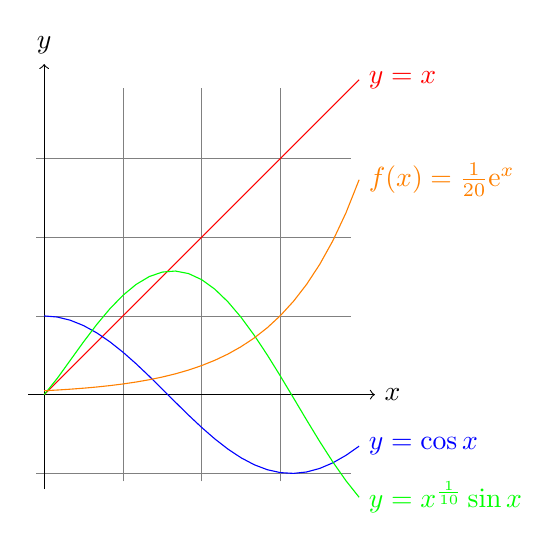
\begin{tikzpicture}[domain=0:4]
  \draw[very thin,color=gray] (-0.1,-1.1) grid (3.9,3.9);
  \draw[->] (-0.2,0) -- (4.2,0) node[right] {$x$};
  \draw[->] (0,-1.2) -- (0,4.2) node[above] {$y$};
  \draw[color=red]     plot (\x,\x)             node[right] {$y =x$};
  % \x r 表示弧度
  \draw[color=blue]    plot (\x,{cos(\x r)})    node[right] {$y = \cos x$};
  \draw[color=green]   plot (\x,{(\x r)^0.1*sin(\x r)})    node[right] {$y = x^{\frac{1}{10}} \sin x$};  
  \draw[color=orange]  plot (\x,{0.05*exp(\x)}) node[right] {$f(x) = \frac{1}{20} \mathrm e^x$};
\end{tikzpicture}
\end{document}
